% !TeX root = ../main.tex

In the topological analysis of scalar fields (SFA), one computes a topological summary capturing qualitative and quantitative shape information from a set of points endowed with a metric and a real-valued function.
That is, we have points with distances and a real number assigned to each point.
More generally, it suffices to have a neighborhood graph identifying the pairs of points within some distance.
% The topological computation often takes the form of persistent homology and integrates local information about the function into global information about its \emph{behavior} as whole.
% In prior work, Chazal et al.~\cite{chazal09analysis} showed that for sufficiently dense samples on sufficiently smooth spaces, the persistence diagram can be computed with some guarantees.
% In followup work, Buchet et al.~\cite{buchet15topological} extended this result to show how to work with noisy inputs.
A fundamental assumption required to have strong guarantees is that the underlying space is sufficiently well-sampled.
In this paper, we show how the TCC can be modified so that one can simultaneously compute the persistence diagram while testing that the underlying space is sufficiently well-sampled.

Initiated by De Silva and Ghrist~\cite{desilva06coordinate,desilva07coverage,desilva07homological}, the theory of homological sensor networks addresses the problem of testing coverage of a bounded domain by a collection of sensors without coordinates.
The main result is the topological coverage criterion, which, in its most general form, states that under reasonable geometric assumptions, the $d$-dimensional relative homology of a pair of simplicial complexes built on the neighborhood graph will be nontrivial if and only if there is sufficient coverage (see Section~\ref{sec:tcc} for the precise statements).
This relative persistent homology test is called the Topological Coverage Criterion (TCC).

Superficially, the methods of SFA and TCC are very similar.
Both construct similar complexes and compute the persistent homology of the homological image of a complex on one scale into that of a larger scale.
They even overlap on some common techniques in their analysis such as the use of the Nerve theorem and the Rips-\v{C}ech interleaving.
However, they differ in some fundamental ways that make them difficult to combine as a single technique.
The main difference is that the TCC requires a clearly defined boundary.
Not only must the underlying space be a bounded subset of $\R^d$, the data must also be labeled to indicate which input points are close to the boundary.
This requirement is perhaps the main reason why the TCC can so rarely be applied in practice.
% Cavanna et al.~\cite{cavanna2017when} generalized the TCC to allow for more general spaces and robust coverage guarantees.
% That work gave a different approach to proving the correctness of the TCC which allows much more freedom in how the boundary is defined.

In applications to data analysis it is more natural to assume that the data measures some unknown function.
% By requiring that our function is related to the metric of the space
We can then replace this requirement with assumptions about the function itself.
Indeed, these assumptions could relate the behavior of the function to the topological boundary of the space.
However, the generalized approach by Cavanna et al.~\cite{cavanna2017when} allows much more freedom in how the boundary is defined.

We consider the case in which we have incomplete data from a particular sublevel set of our function.
% We consider the case where we can only verify our sample in a part of the  % have incomplete data from a particular sublevel set of our function.
Our goal is to isolate this data so we can analyze the function in only the verified region.
%corresponding part persistent homology of the function in the verified region without allowing missing
From this perspective, the TCC confirms that we not only have coverage, but that the sample we have is topologically representative of the region near, and above this sublevel set.
We can then re-use the same machinery to analyze a \emph{part} of the function in a specific way.

\begin{figure}[htbp]
  \centering
  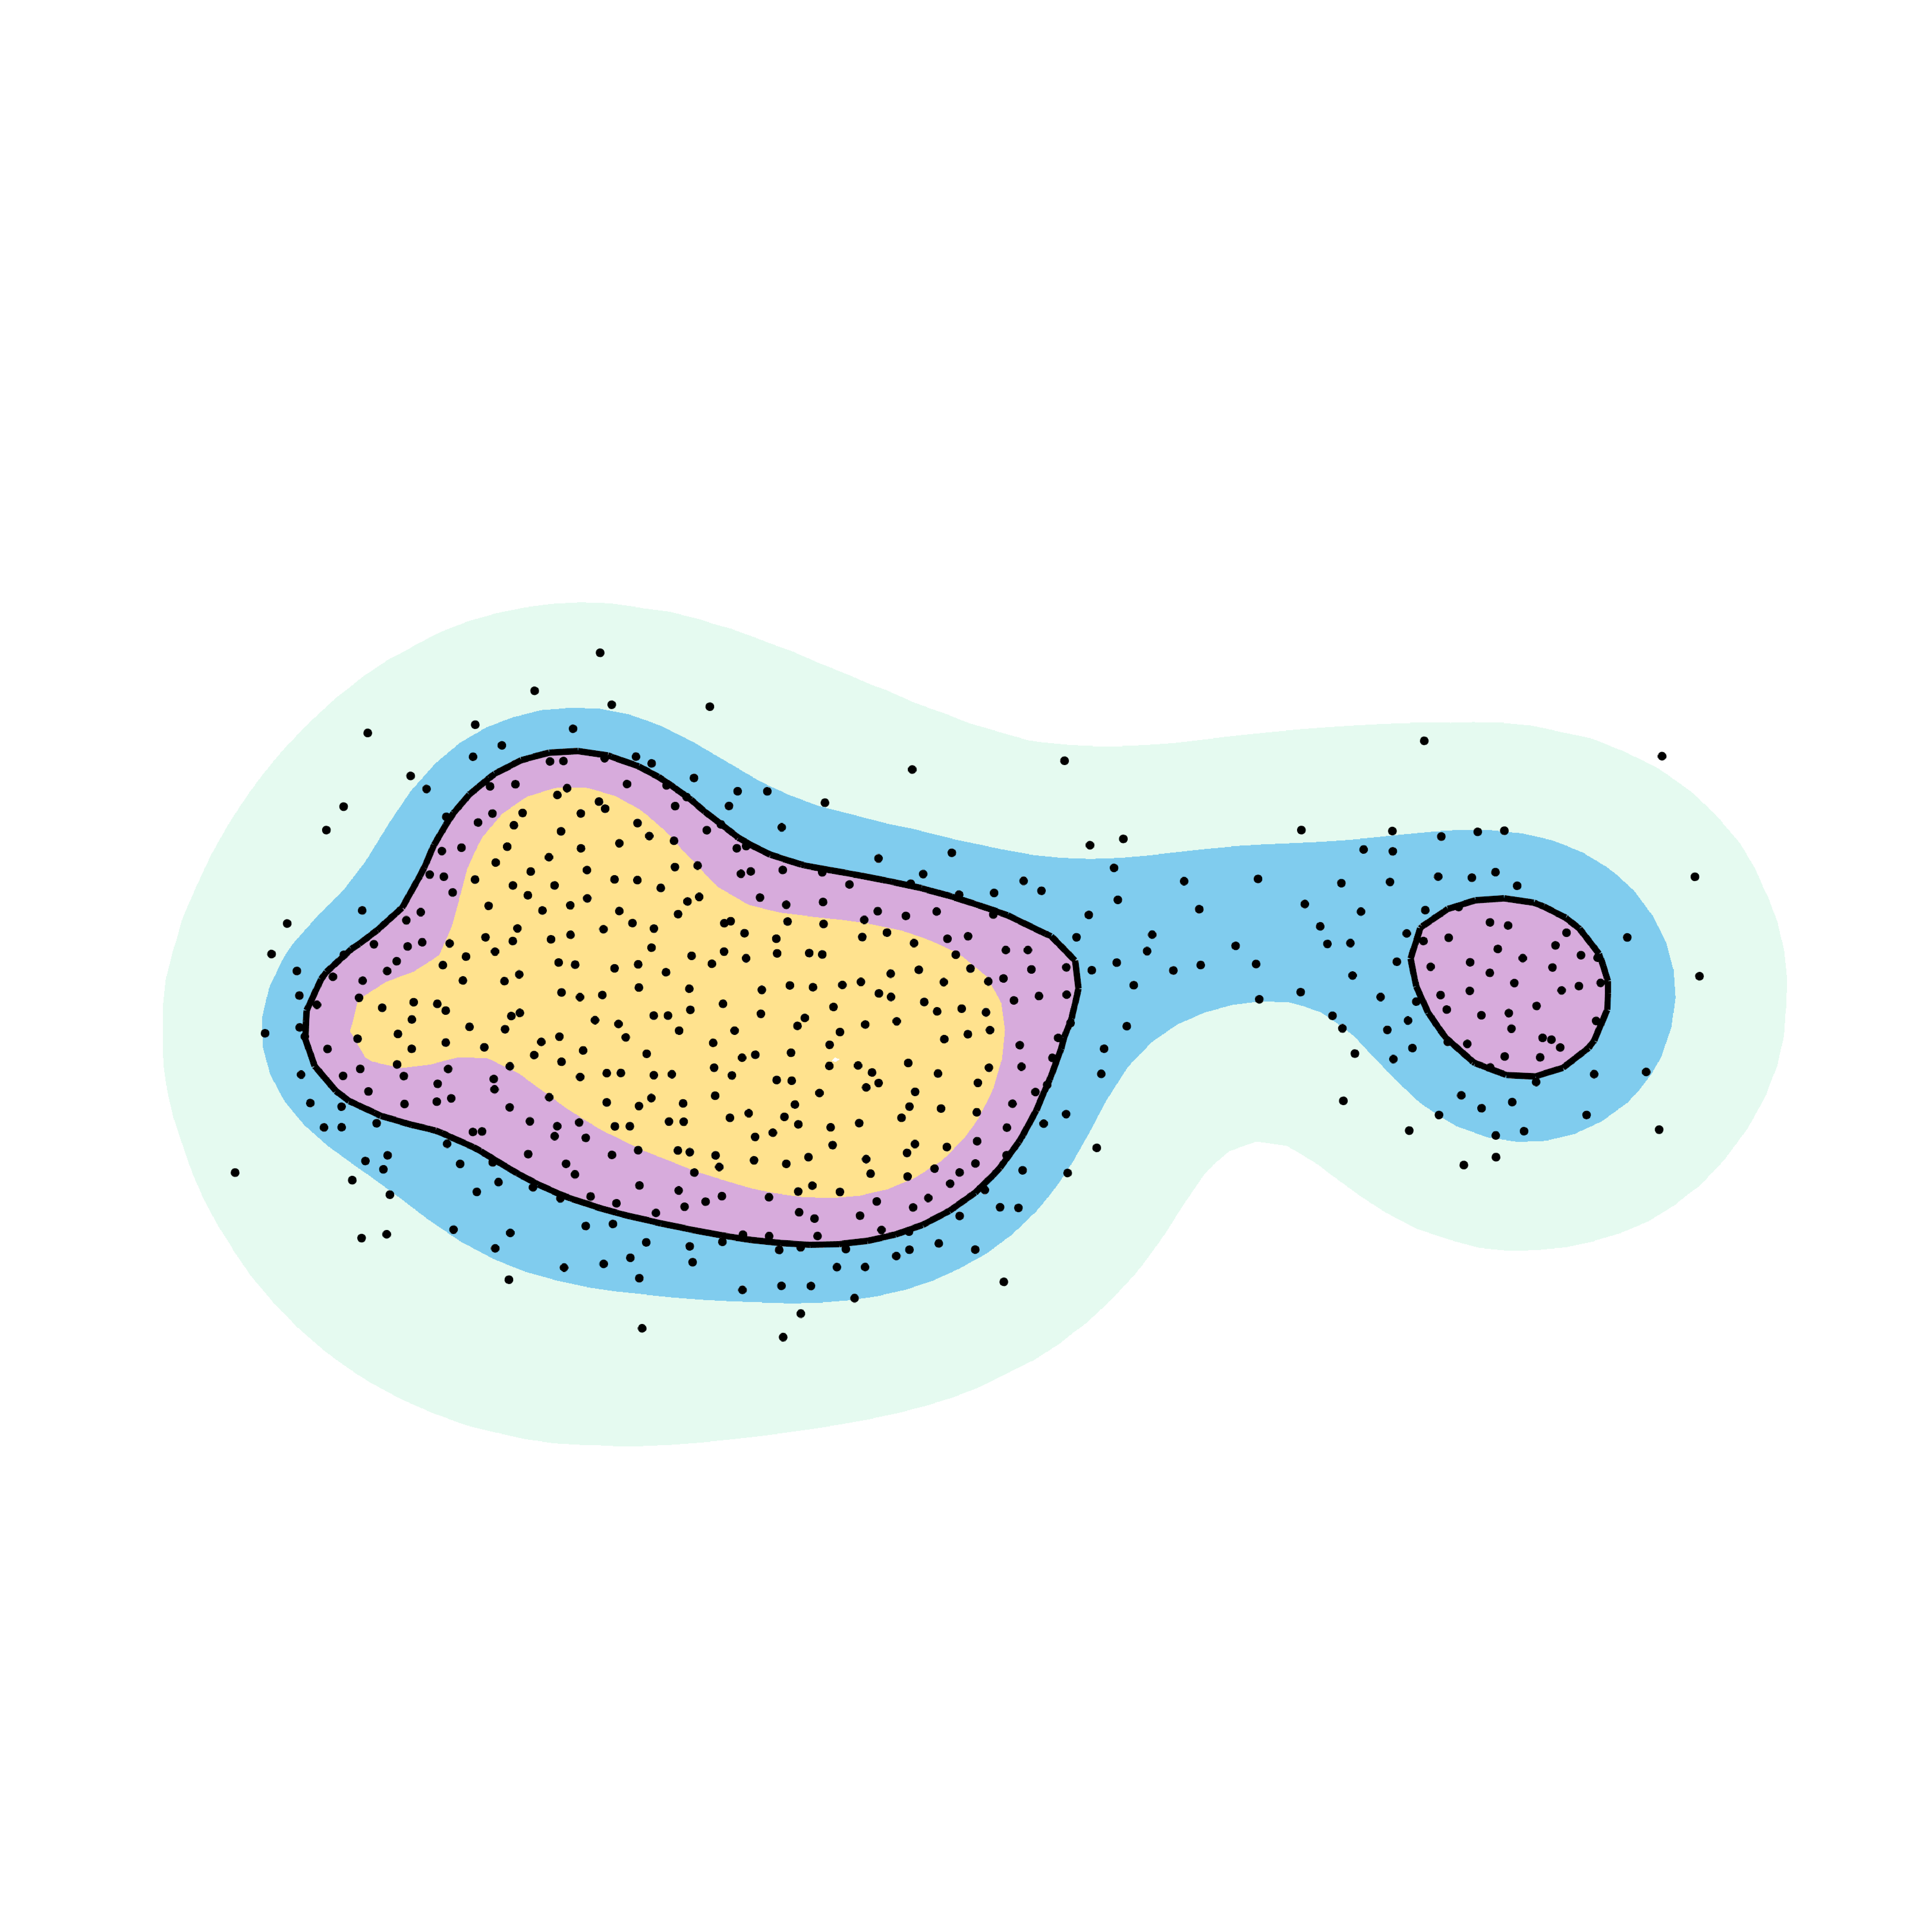
\includegraphics[trim=0 500 0 500, clip, width=0.45\textwidth]{figures/samples/samples}
  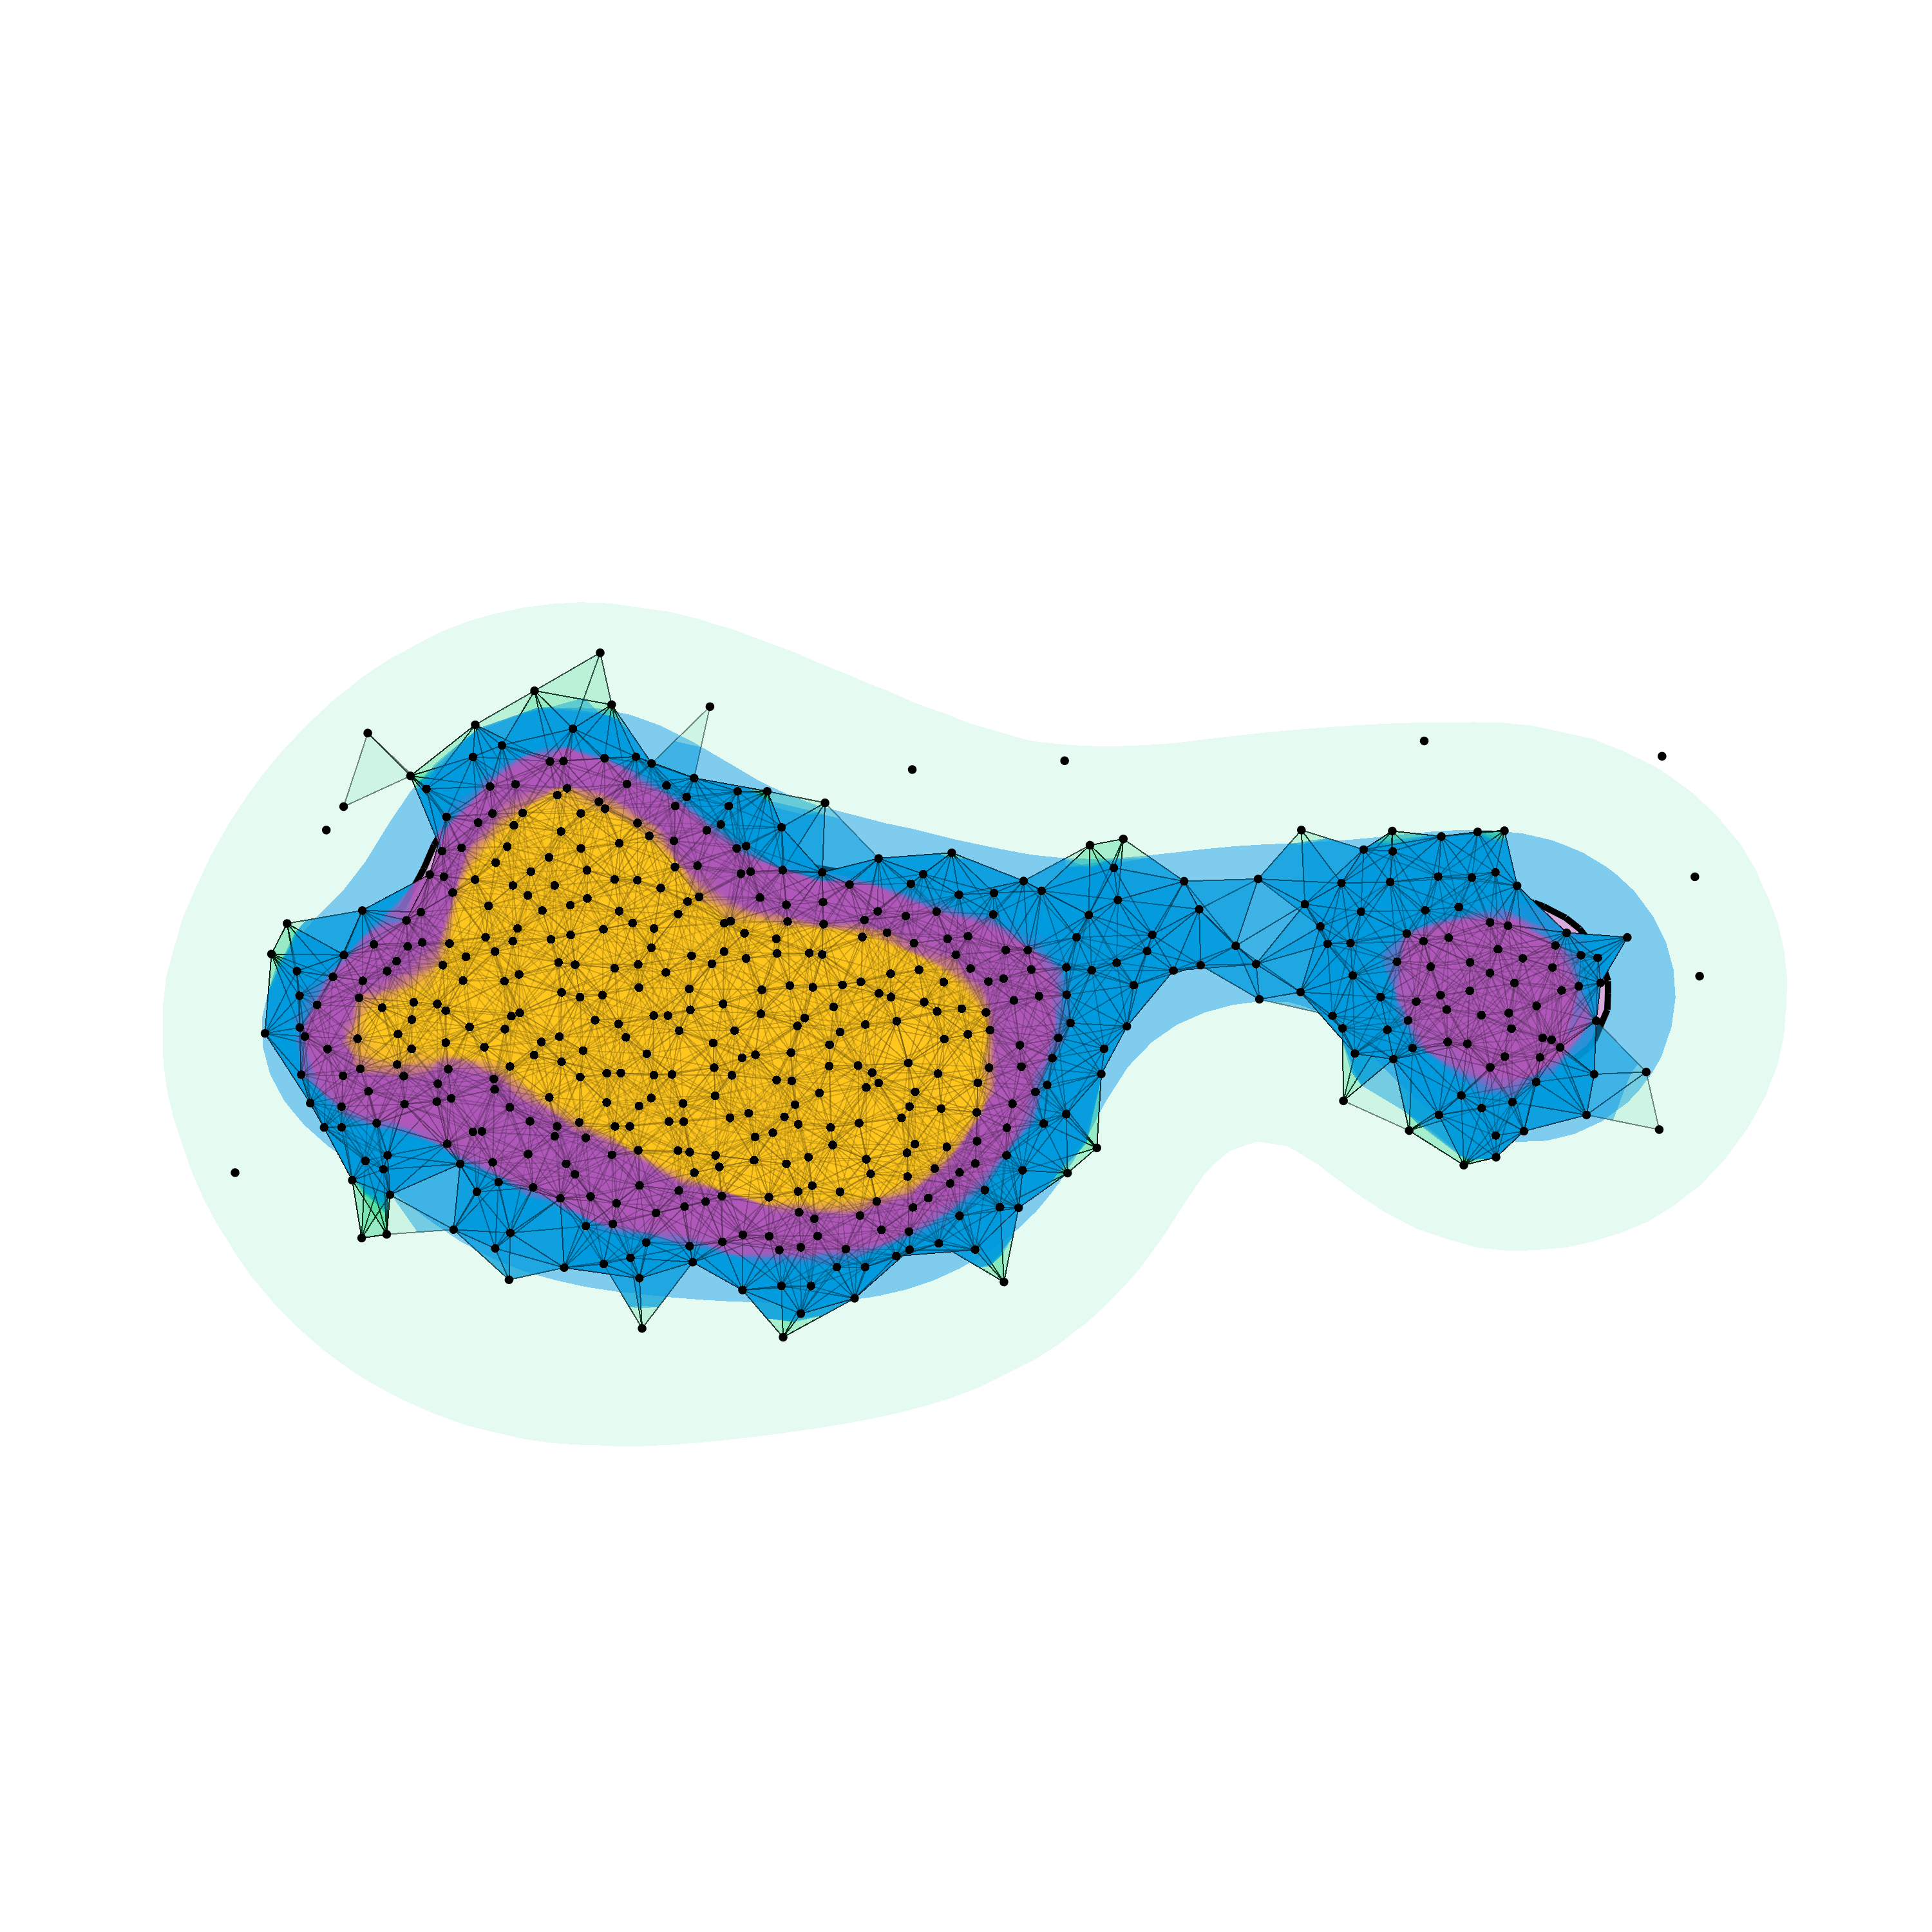
\includegraphics[trim=0 500 0 500, clip, width=0.45\textwidth]{figures/samples/scalar1}
  \caption{A partially sampled scalar field.}\label{fig:main}
\end{figure}
